% \documentclass[12pt]{article}

%%v helpful MIT exam schema, see http://www-math.mit.edu/~psh/exam/examdoc.pdf
 \documentclass[9pt]{exam} 
% \qformat{\textbf{Question \thequestion}\quad \thepoints\hfill } % Large depth to make space}
 \renewcommand{\thesubpart}{(\roman{subpart})}
 \renewcommand{\subpartlabel}{\thesubpart}
 \footer{}{}{Page \thepage\ de \numpages}
\addpoints
% \pointsinmargin
% \boxedpoints
%\renewcommand{\questionshook}{\setlength{\itemsep}{1cm}}
%\renewcommand{\partshook}{
%	\setlength{\itemsep}{0.5cm}
%    	\setlength{\leftmargin}{-10pt}%
%}

\usepackage{cmbright}

\pagestyle{empty} %for handouts
\addtolength{\jot}{2em} % this makes all formulae a bit more spaced vertically for handouts
\setlength{\parindent}{0pt} %we're not writing a novel
%\renewcommand{\arraystretch}{2} %makes tables taller, so easier to write in

\usepackage[fleqn]{amsmath}
\usepackage{amssymb} %standard classy maths symbols
\usepackage[a4paper, margin=1in]{geometry} %makes it easy to specify where to put stuff on the page

\usepackage{siunitx} %v handy way of getting SI units to typeset correctly...
\sisetup{locale = FR} %... and now it will use a comma for decimals

\usepackage[utf8]{inputenc}

% \usepackage[french]{babel} % frenchify everything (e.g. a Table becomes a Tableau)
\usepackage{lmodern} % font with nicer French characters than standard
\usepackage{textcomp} % and more help for special characters

\usepackage{tcolorbox} % basic but good package for boxes around text
\tcbset{colback=black!5!white}
\usepackage{color} % colours
%\newcommand{\fillin}{\color{black!1!white}} %makes the text disappear
%\definecolor{fillin}{rgb} {1.00,1.00,1.00}
%\renewcommand{\fillin}{\color{blue}} \definecolor{fillin}{rgb} {0.00,0.00,1.00} %makes the filling in text appear (in blue)

\usepackage{enumitem} % can change the labels on lists, items, enumerates

\usepackage{tikz, pgfplots} % interval diagrams, sets, etc.
\usetikzlibrary{calc,trees,positioning,arrows,fit,shapes}

\begin{document}
\sffamily

\textbf{Name:} \dotfill

\


In the sketch we have $P(-2,-1)$. The gradient of $[PQ]$ is 2. 
\vspace{-3mm}
\begin{center}
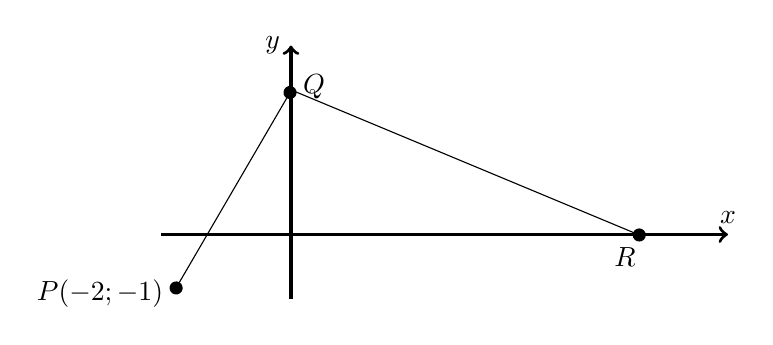
\begin{tikzpicture}[scale=0.75]

\draw[very thick, ->] (-2.2,0) -- (7.4,0) node[above] {$x$};
\draw[very thick, ->] (0,-1.1) -- (0,3.2) node[left] {$y$};

\draw[*-*] (-2,-1) node[left] {$P(-2; -1)$} -- (0.04,2.5)  node[right] {$Q$};
\draw[-*] (0,2.45)-- (6,-0.05)  node[below left] {$R$};

\end{tikzpicture}
\end{center}

\begin{questions}
\question[1] Give the formula for the gradient between two points $(x_1, y_1)$ and $(x_2, y_2)$.
\fillwithdottedlines{21mm}

\question[3] Given that $Q$ lies on the $y$-axis, find the coordinates of $Q$.
\fillwithdottedlines{21mm}



\question[4] Given that  and $(PQ) \perp (QR)$ and that $R$ lies on the $x$-axis, find the coordinates of $R$.
\fillwithdottedlines{\stretch{1}}

\question \textbf{Bonus.} Find the coordinates of the point $S$ in the first quadrant which satisfies $\overline{QS} = 3$ and $\overline{RS} = 6$.

\emph{Work overleaf, then write your answer here.}
\fillwithdottedlines{10mm}

\end{questions}

\begin{tcolorbox}

\textbf{Name of marker:}

\begin{center}
\gradetable[h][questions]
\end{center}

\end{tcolorbox}


\end{document}